%\documentclass{article} %[twocolumn]
\documentclass[AMA,STIX1COL]{WileyNJD-v2}

\articletype{Main paper}%

%\usepackage{algorithmic}
\usepackage{algorithm}
\usepackage{algorithmicx}
\usepackage{algpseudocode}
\usepackage{booktabs}
\usepackage{array}
\usepackage{graphicx}
\usepackage{amsmath}
\usepackage{amsfonts}
\usepackage{amssymb}
\usepackage{multirow}
\usepackage{url}

\received{26 April 2016}
\revised{6 June 2016}
\accepted{6 June 2016}

\begin{document}

\title{A hypothesis test of feasibility for external pilot trials assessing recruitment, follow-up and adherence rates}

\author[CTRU]{Duncan T. Wilson*}
\author[CTRU]{Rebecca E. A. Walwyn}
\author[CTRU]{Julia Brown}
\author[CTRU]{Amanda J. Farrin}

\authormark{Wilson \textsc{et al.}}

\address[CTRU]{Leeds Institute of Clinical Trials Research, University of Leeds, Leeds, UK}

\corres{Duncan T. Wilson, Clinical Trials Research Unit, Leeds Institute of Clinical Trials Research, University of Leeds, Leeds, LS2 9JT.
\email{d.t.wilson@leeds.ac.uk}}

\abstract{
% 250 word limit
\textbf{Background}: The power of a large clinical trial can be adversely affected by low recruitment, follow-up and adherence rates. External pilot trials, conducted before a planned definitive trial but on a smaller scale, can be used to estimate these parameters and identify any issues. Pilot trials commonly specify decisions rules which use these estimates to determine if the definitive trial is feasible and should go ahead, but there is little methodological research underpinning how they, or the pilot sample size, should be chosen.

\textbf{Methods}: We propose that the feasibility of a definitive clinical trial should be assessed using a statistical test of the associated pilot trial data. We argue that recruitment, follow-up and adherence rates are of interest primarily in how they affect the power of the definitive trial, and so use power as a measure of feasibility. Focussing on the common scenario of a two-arm parallel group definitive trial with a single normally distributed primary endpoint, we show how hypotheses for this test can be defined. We suggest a test statistic and provide its sampling distribution, thus defining type I and II error rates, and show how these can be calculated and used to inform the pilot trial sample size and progression decisions. We then extend our formulation to include estimating the standard deviation of the primary endpoint.

\textbf{Illustration}: We use our method to re-design the TIGA-CUB trial, a pilot trial comparing a psychotherapy with treatment as usual for children with conduct disorders. Our results show that reasonable error rates for the pilot can be obtained without inflating its sample size, and that the standard practice of applying several independent progression criteria is substantially less efficient.
% Think about what we want to emphasise as the key messages throughout. We aren't saying that we can just carry on as normal with the simple rules-of-thumb - we are showing that a careful statistical asessment should be used to find the most appropriate design.

\textbf{Conclusions}: The proposed hypothesis test can substantially improve the quality of decision making following an external pilot trial in comparison to current standard practice, whilst maintaining the pilot sample size at typical levels.
}

% Up to 6 keywords
\keywords{Pilot trials, sample size}

\maketitle

\section{Introduction}\label{sec:intro}

Randomised Controlled Trials (RCTs) often fail to recruit to target \cite{Sully2013}, leading to an analysis with less power than intended. Power can also be adversely affected by unexpectedly large rates of attrition, poor adherence to the allocated treatment \cite{Fay2006}, and incorrect specification of a nuisance parameter such as the standard deviation of a continuous endpoint \cite{Teare2014}. A common approach to anticipatethese problems is to run a small version of the intended trial, known as an external pilot trial, to obtain estimates of the relevant parameters and decide if, and how, a larger `definitive' trial should be conducted  \cite{Eldridge2016}. This decision is typically made with reference to so-called \emph{Progression Criteria} (PCs), a set of conditions which must be satisfied for the definitive trial to be considered feasible \cite{Avery2017}. In the case of quantitative PCs such as those pertaining to recruitment rate, parameter estimates are computed using the pilot data and then compared against threshold values. If all estimates exceed their respective thresholds, it is recommended that the definitive trial should be conducted. A recent workshop identified that recruitment, follow-up, and intervention adherence have emerged as common targets of progression criteria \cite{Avery2017}. 

The increasing use of pilot trials has led to several clarifications regarding their definition, design and conduct \cite{Lancaster2004, Craig2008, Arain2010, Thabane2010, Eldridge2016}; an extension to the CONSORT statement \cite{Eldridge2016a}; and a dedicated journal \cite{Lancaster2015}. Despite this, there is little methodological research available to help researchers choose appropriate progression criteria \cite{Avery2017}. Estimates computed using the small samples available in pilots can suffer from substantial imprecision \cite{Cooper2018}, leading to the meeting or missing of PCs by chance alone \cite{Eldridge2015}. One suggested solution has been to specify two threshold values corresponding to hard `stop' and `go' decisions for each PC \cite{Avery2017}. If an estimate falls between these thresholds an intermediate `modify' decision is suggested, providing the flexibility to argue that the definitive trial will in fact be feasible providing some modifications are made to the intervention or the trial protocol in response to what was observed in the pilot. Although increasingly common \cite{Eldridge2016a}, it is not clear how such thresholds should be pre-specified (as required by the NIHR, a major funder of pilot trials in the UK \cite{NIHR2017}) when it will in general be impossible to know the magnitude of possible improvements until after the pilot has been conducted. We therefore focus on making a binary stop/go decision after the pilot trial.

% Needs more clarification RE the three outcome approach. Avoid discounting it entirely and return to it in the discussion?

Closely related to the choice of PCs is the choice of pilot trial sample size, which determines the level of sampling variability in the pilot estimates. Methods for determining pilot trial sample size have generally focussed on obtaining a sufficiently precise estimate of the standard deviation of a continuous primary outcome to inform the sample size calculation of the definitive trial \cite{Browne1995, Julious2005, Sim2012, Teare2014, Eldridge2015, Whitehead2015}. These methods are nevertheless widely used to choose pilot sample size even in cases where the estimation of the standard deviation is not the only, or primary, objective. In doing so, the methods are typically reduced to simple rules-of-thumb, such as requiring 35 participants in each arm \cite{Teare2014}. However, there is no reason to believe this will be the optimal choice for other objectives in pilot trials, including the estimation of recruitment, follow-up and adherence rates. For example, using a sample size of 35 participants to estimate a true rate of adherence in the intervention arm of 0.8 would lead to an approximate 2-sided 95\% confidence interval around the estimate of width 0.27. By choosing both the pilot sample size and the progression criteria without a formal analysis of their resulting statistical properties we risk designing pilots which are unlikely to lead to a `go' decision even when there are no underlying problems; or conversely, unlikely to identify truly infeasible situations before proceeding to the definitive trial.

% As a way to design, we have power or precision arguments. Precision is common in practice, although no guidance as to how to choose n - we use a rule of thumb, then show the CI widthc we would expect, and use that as a justification for n (ref Julious, justification needed but not necesarily a calculation?). So the shortcoming of precision argument is - how precisise is enough? Power does the next step, connecting the precision of estimates to the propoerties of the stop go decision that will be made based on them. So particularly appropriate for early phase studies, where this decision is very explicit and will be made. Note that (PC aside) we will likely have some implicit decision rule in mind, involving comparing CI limits with null and alternative values. But these are equivalent to a test formulation - again, Cocks method is presented in CIs, but can be more explicitly formulated as a test.

An alternative approach to choosing the progression criteria and pilot sample size is to use a hypothesis testing framework. If researchers can describe appropriate null and alternative hypotheses, they can choose the pilot sample size and PCs based on the resulting type I and II error rates. Despite hypothesis testing being the standard method for the design and analysis of early phase trials in the drug setting (known as `phase II' trials), it is rarely used in pilot trials \cite{Eldridge2016a}. Concerns about such tests having low power due to the small sample size of the pilot have been voiced repeatedly \cite{Lancaster2004, Arain2010, Thabane2010, Eldridge2015}, leading to some authors suggesting inflating the type I error rate used in the test to maintain reasonable power \cite{Cocks2013, Lee2014}. Concerns about power are further justified in pilot trials if several hypothesis tests are applied independently to several endpoints (such as recruitment, follow-up and adherence) and a `go' decision reached only if all results are positive, a procedure which will suffer from the `reverse-multiplicity' problem \cite{Senn2007, Chuang-Stein2007}. Other approaches to testing include methods which explicitly allow for trade-offs between different parameters to be acknowledged \cite{Conaway1996, Thall2008}, a feature commonly seen in pilot trials \cite{Wilson2015}.

In this paper we develop a hypothesis test for external pilot trials assessing recruitment, follow-up and adherence rates to make progression decisions to a planned definitive trial which will use a continuous, normally distributed primary endpoint. We argue that the power of the definitive trial, as a function of these three parameters, can be used as a univariate measure of its feasibility. We propose a test statistic and show how it can be used in a hypothesis testing framework, leading to type I and II error rates for the pilot trial which can help us choose the pilot sample size and progression criteria. We compare our method with current practice and show how the latter can be substantially worse in comparison. We then extend our formulation to include estimation of the standard deviation nuisance parameter.

% Make the connection with the phase II literature explicit. Testing is standard there as a way to design and analyse, although almost always on efficacy only. General methods for two endpoints have been proposed and are used a lot for efficacy and toxicity, but they have clear shortcomings for us (not lease that we have three endpoints, and particularly the reverse multiplicity problem and inoring trade-offs). What else can we take? Common to relax type I error to maintain a small phase II sample. Connect back to pilot literature where this has also been proposed explicitly \cite{Lee2014}, and implicitly in~\cite{Cocks2013} whose argument is presented in terms of confidence intervals, but is equivalent to powering for a test with 0.5 alpha.

% Some examples of not sticking to PC - WATCH-IT, where they thought the "red" flag was a fluke and ignored it? Expect flexibility, but equally if the PC are not thought reliable guides to decision making, why bother specifying them?

% Note that we ask for the definitive trial sample size to be chosen prior to the pilot - but this is fine and in line with current uidance, where funders expect to see a clear plan in advance.

% Shout here that we are considering a frequentist approach

\section{Problem}\label{sec:problem}

We consider an external pilot trial which is being conducted in advance of a large two-arm parallel group trial comparing an intervention with a control with respect to a normally distributed primary outcome. Initially, we will assume the standard deviation of the outcome (constant between arms) is known, though this will be relaxed in Section \ref{sec:extension}. The pilot trial will take the form of a smaller version of the definitive trial. 

We assume the design of the definitive trial to be fixed prior to the pilot. In particular, we assume that the target sample size of the definitive trial, denoted $n_t$, is known. We also know the number of eligible participants who will be approached to take part in the definitive trial, $n_e$ (following from knowing the time-scale of the trial and the incidence / presentation rate). The definitive trial will continue to recruit until either the target sample is obtained, or the number of eligible participants is exhausted. The pilot trial will assess the recruitment, follow-up, and adherence rates which will govern the definitive trial. Recruitment rate is defined as the proportion of those approached to take part in the trial who consent. Follow-up rate is the proportion of those participants who consent who provide primary outcome data. Adherence rate is defined as the proportion of those participants who consent and are randomised to the intervention arm who meet some adherence criteria, such as attending a minimal number of treatment sessions. 

Our goal is to describe a parametric form of decision rule that can be used after the external pilot trial to make a stop/go decision, and to provide a way to evaluate the statistical property of any such rule for any choice of pilot trial sample size.

\section{Proposed hypothesis test of feasibility}\label{sec:methods}

The general strategy we use is as follows. We define the feasibility of the definitive trial with respect to the power it will have to detect a minimal clinically important difference when it exists, a function of the true recruitment, follow-up and adherence rates. Denoting these parameters by $\phi$ and the power function by $g(\phi)$, we then define two subspaces of the parameter space $\Phi$:
\begin{align*}
\Phi_0 = \{\phi \in \Phi ~ | ~ g(\phi) <= p_0 \}; \\
\Phi_1 = \{\phi \in \Phi ~ | ~ g(\phi) >= p_1 \}.
\end{align*}
That is, $\Phi_0$ is the set of all parameter values which would lead to the definitive trial having a power of $p_0$ or less. We will refer to $\Phi_0$ as the null hypothesis. The alternative hypothesis $\Phi_1$ is the set of all parameter values leading to the definitive trial having a power of at least $p_1$. The threshold values $p_0, p_1$ are chosen such that if $\phi \in \Phi_0$ we would like to control the probability of mistakenly proceeding to the definitive trial (a type I error). Similarly, if $\phi \in \Phi_1$ then we would like to control the probability of mistakenly discarding the intervention (a type II error).

Testing feasibility in the pilot trial will involve calculating a statistic $s(\hat{\phi})$ based on the pilot estimate $\hat{\phi}$ and proceeding to the definitive trial if and only if it exceeds some pre-specified  critical value $c$. We can then define the type I and II error rates of the pilot trial:
\begin{align}\label{eqn:ocs}
\alpha = \max_{\phi \in \Phi_0} Pr[ s(\hat{\phi}) > c ~ | ~ \phi], \\
\beta = \max_{\phi \in \Phi_1} Pr[ s(\hat{\phi}) < c ~ | ~ \phi].
\end{align}

In the remainder of this section we will describe the relevant power function $g(\phi)$, a statistic $s(\hat{\phi})$ and its sampling distribution in the pilot, and a way to calculate the error rates resulting from specific choices of pilot sample size $n_p$ and critical value $c$.

\subsection{Power of the definitive trial}\label{sec:power}

\begin{table}
\centering
\caption{Notation.}
\begin{tabular}{l p{8cm}}
\toprule
$\phi_r$ & Recruitment rate \\
$\phi_a$ & Adherence rate \\
$\phi_f$ & Follow-up rate \\
$\phi$ & $(\phi_r, \phi_a, \phi_f)$ \\
$n_e$ & number of eligible participants expected to be approach for consent \\
$n_t$ & target sample size (per arm) of the definitive trial \\
$\mu$ & Between group difference \\
$t_i$ & Binary treatment arm indicator for participant $i$ \\
$a_i$ & Binary treatment adherence indicator for participant $i$ \\
$\bar{Y}_j$ & Mean response in arm $j$ \\
$C$ & Number of consenting participants (per arm) \\
$R$ & Number of successfully recruited participants (per arm) \\
$F_j$ & Number of participants successfully followed-up in arm $j$ \\
$A$ & Number of participants who adhere to treatment in the intervention arm \\
$g(\phi)$ & Power of the definitive trial conditional on $\phi$ \\
$R_p^-$ & Number of eligible participants who do not consent to the pilot trial \\
$h(n_p, c, \phi)$ & Power of the pilot trial with $n_p$ participants in each arm, critical value $c$, and conditional on $\phi$ \\
\bottomrule
\end{tabular}
\end{table}

Recall that recruitment in the definitive trial will continue until either all $n_e$ eligible participants have been approached, or until $r = n_t$. For each eligible participant, the probability of consenting is denoted $\phi_r$. For each recruited participant, the probability of successful follow-up is denoted $\phi_f$. And for each participant in the intervention arm who is successfully followed-up, the probability of them adhering to the intervention is denoted $\phi_a$. We assume that adherence is absolute, in the sense that no treatment effect is obtained for non-adherers. The continuous primary outcome for patient $i$ can be modelled as
$$
y_i = t_i a_i \mu + e_i,
$$
where $t_i$ and $a_i$ are binary indicators of treatment arm and adherence respectively, $e_i \sim N(0, \sigma^2)$ is the residual term, and we have committed the usual constant intercept for notational simplicity and without loss of generality.

Power in the definitive trial is determined by the sampling distribution of the difference in group means, $\bar{Y}_1 - \bar{Y}_0$. We assume that the definitive trial per-arm sample size is greater than 30, allowing the sampling distributions of the group sample means to be approximated by normal distributions. The sample means are
\begin{align*}
\bar{Y}_1 &= \frac{A}{F_1}\mu + \frac{1}{F_1} \sum_{i=1}^{F_1} e_i, \\
\bar{Y}_0 &= \frac{1}{F_0}\sum_{i=1}^{F_0} e_i,
\end{align*}
where $F_j$ denotes the number of participants in arm $j$ who are followed-up, and $A$ denotes the number of participants in the intervention arm who both adhere \emph{and} are follow-up. These sample means have expectations $E[\bar{Y}_1 | \phi] = E[\frac{A}{F_1}\mu | \phi] = \phi_a \mu$ and $E[\bar{Y}_0 | \phi]$. The appendix will show that
\begin{align}\label{eqn:vars}
Var(\bar{Y}_1) &= \frac{\sigma^2}{\phi_f E[R]} + \frac{\mu^2}{\phi_f E[R]} \phi_a (1-\phi_a), \\
Var(\bar{Y}_0) &= \frac{\sigma^2}{\phi_f E[R]}.
\end{align}
The power of the trial can then be obtained by substituting the expectation and variance of the sample means into the usual formula (which, again, assumes they are normally distributed):
\begin{align*}
g(\phi) &= \Phi \left(\frac{E[\bar{Y}_1 - \bar{Y}_0]}{\sqrt{Var(\bar{Y}_1 - \bar{Y}_0)}} - z_{1-\alpha} \right) \\
&= \Phi \left( \frac{\phi_a\mu}{\sqrt{ \frac{\sigma^2}{\phi_f E[R]} + \frac{\mu^2}{\phi_f E[R]} \phi_a (1-\phi_a) + \frac{\sigma^2}{\phi_f E[R]}} } - z_{1-\alpha} \right) \\
&= \Phi \left( \frac{ \phi_a\mu \sqrt{\phi_f E[R]} } {\sqrt{2\sigma^2 + \mu^2 \phi_a(1-\phi_a)}} - z_{1-\alpha} \right) \\
&= \Phi \left( x(\phi) - z_{1-\alpha} \right),
\end{align*}
where 
$$
x(\phi) =  \frac{ \phi_a\mu \sqrt{\phi_f E[R]} } {\sqrt{2\sigma^2 + \mu^2 \phi_a(1-\phi_a)}}.
$$
We can now define our hypotheses as
\begin{align*}
\Phi_0 &= \{\phi ~ | ~ x(\phi) <= x_0 \} \\
\Phi_1 &= \{\phi ~ | ~ x(\phi) >= x_1 \},
\end{align*}
where 
$$
x_i = \Phi^{-1}(p_i) + z_{1-\alpha} \text{ for } i = 0,1.
$$

%Note that the majority of the difference in power comes from the numerator. The denominator differs from the usual by the term $\mu^2\phi_a(1-\phi_a)$, which increases with $\mu$ and as $\phi_a \rightarrow 0.5$. But note that
%$$
%\frac{\mu^2\phi_a(1-\phi_a)}{2\sigma^2} = \frac{\phi_a(1-\phi_a)}{2} \left( \frac{\mu}{\sigma} \right)^2,
%$$
%so for example when the standardised difference to detect is 0.3, the second term is at most 1.125\% of the usual and so won't be hugely influential.

%Clearly, $x(\phi)$ is non-injective, so there will be a set of points $\phi$ which lie on the boundaries of these spaces with $x(\phi) = x_i$.

\subsection{Pilot test statistic and sampling distribution}

A natural choice of statistic is $s(\hat{\phi}) = x(\hat{\phi})$ [RW - in words as well]. To determine its sampling distribution we must first clarify the sampling model of the pilot trial. We assume that screening of participants will continue until the number who have consented reaches a target value of $2n_p$. This means that the number of eligible participants who do \emph{not} consent, $R_p^-$, follows a negative binomial distribution with parameter $\phi_r$. 

In the intervention arm, we allow for correlated follow-up and adherence outcomes by using a multinomial model [Why? what are the alternatives?]. We use the notation $p_{11}$ to denote the probability a participant will both adhere and be followed up; $p_{10}$ to denote adherence but loss to follow-up; and similarly for $p_{01}$ and $p_{00}$. We specify the model in terms of the conditional probability of adherence given follow-up, $\phi_a = p_{11}/(p_{11} + p_{01})$; overall probability of follow-up, $\phi_f = p_{01} + p_{11}$; and the odds ratio $\phi_{OR} = p_{00}p_{11}/p_{01}p_{10}$. These inputs translate into the following probabilities:
\begin{align*}
p_{11} &= \phi_a \phi_f \\
p_{01} &= \phi_f - p_11 \\
p_{00} &= \frac{\phi_{OR} p_{01}(1-p_{11}-p_{01})}{p_{11} + \phi_{OR} p_{01}} \\
p_{10} &= 1 - p_{11} - p_{01} - p_{00}.
\end{align*}

% We can put this in the appendix, as its only really important as a way to allow the user to specify their problem using this parameterisation.

Let $n_{af} = (n_{11}, n_{10}, n_{01}, n_{00})$ be the numbers of participants in each cell of the contingency table and $\mathcal{N}_{af}$ be the set of possible realisations of these numbers in the pilot trial. Under this model, the power of a pilot with $n_p$ participants in each arm, critical value $c$, and true parameter values $\phi$, is approximately
\begin{align}\label{eqn:pilot_pow}
h(n_p, c, \phi) &= \sum_{n_{af} \in \mathcal{N}_{af}} \left( \sum_{r^- = 0}^{r^-_{max}} 
I \left[ x(\hat{\phi}) > c \mid  r^-, n_{af}, \phi \right] p_{r^-}(r^- | n_{af}, \phi) \right)     
p_{af}(n_{af} |\phi),
\end{align}
where $p_{af}(.)$ is the multinomial density with parameter $(p_{11}, p_{01}, p_{10}, p_{00})$ and  $p_{r^-}(.)$ is the negative binomial density with parameter $\phi_r$. The approximation comes from the inner summation term over the number of eligible participants who do not consent being limited to a finite $r^-_{max}$. We set  $r^-_{max}$ to the upper 0.999 quantile of the negative binomial distribution, ensuring an accurate approximation whilst avoiding excessive computation.

When it can be assumed that adherence and follow-up outcomes are independent, equation \ref{eqn:pilot_pow} simplifies to
\begin{equation*}
h(n_p, c, \phi) = \sum_{a=0}^{n_p} \left[  \sum_{f=0}^{2n_p} \left( \sum_{r^- = 0}^{r^-_{max}} 
I \left[ x(\hat{\phi}) > c \mid  r^-, n_{af}, \phi \right] p_{r^-}(r^- | n_{af}, \phi) \right) p_{f}(f |\phi)  \right] p_a(a | \phi).
\end{equation*}
This reduces the number of terms to be summed, and thus decreases computational time. [RW - when would this assumption be reasonable in practice?] [What are the implications? In discussion and in the appendix examples, need to give an indication of how much longer the computations are when we have the more general case]

%Under this model, the power of a pilot trial with $n_p$ participants in each arm, critical value $c$, and true parameter values $\phi$, is
%\begin{align}
%g(n_p, c, \phi) &= \sum_{a = 1}^{n_p} \left( \sum_{f = 1}^{2n_p} 
%Pr \left[ \hat{\phi}_r \hat{\phi}_f \hat{\phi}_a^2 > c \mid f, a, \phi \right]    
%f_f(f | a, \phi) \right) f_a(a | \phi) \\
%&= \sum_{a = 1}^{n_p} \left( \sum_{f = 1}^{2n_p} 
%Pr\left[ \frac{2n_p}{r_{-} + 2n_p} \frac{f}{2n_p} \frac{a^2}{n_p^2} > c \mid f, a, \phi \right]    
%f_f(f | a, \phi) \right) f_a(a | \phi) \\
%&= \sum_{a = 1}^{n_p} \left( \sum_{f = 1}^{2n_p} F_{r_-} \left( \left\lfloor\frac{a^2f}{n_p^2c} \right\rfloor - 2n_p \mid f,a,\phi \right)  f_f(f | \phi) \right) f_a(a | \phi)
%\end{align}

%In the above we assumed that the number of adherers and the number of follow-ups are independent. We might argue that this won't be the case - an individual who sticks to the protocol is more likely to also stick with the trial and give the follow-up data. This won't be any more complicated as we can easily put the joint distribution into the above, but we will have an extra nuisance parameter in the correlation. We can start by assuming this is known. From above we know that we only need 2 out of the 3 necessary parameters of the joint distribution to define our hypotheses. 

\subsection{Operating characteristics}\label{sec:ocs}

Recall that the type I (II) error rate of the pilot trial is defined as the largest probability of proceeding (failing to proceed) to the definitive trial when the true parameter is in the null (alternative) hypothesis. That is, 
\begin{align*}
\alpha(n_p, c) &= \max_{\phi \in \Phi_0} ~ h(n_p, c, \phi) , \\
\beta(n_p, c) &= \max_{\phi \in \Phi_1}  ~ 1 - h(n_p, c, \phi).
\end{align*}
Designing a pilot trial could proceed by considering a set of candidate sample size values $n_p$ and for each, $\alpha(n_p, c)$ and $\beta(n_p, c)$ for a range of possible critical values $c$, plotting the operating characteristic curves obtained for each $n_p$, and then choosing the $(n_p, c)$ pair which is deemed to give the best balance between the costs of sampling and the two types of errors. 

An alternative formulation is to (for fixed $n_p$) cast the problem as one of constrained bi-objective optimisation over the space $\mathbb{R} \times \Phi \times \Phi$, simultaneously searching for a critical value $c$ and two points in the parameters space, $\phi_0$ and $\phi_1$, which maximise type I and II error rates whilst satisfying the constraints that $\phi_0 \in \Phi_0$ and $\phi_1 \in \Phi_1$. Formally, we solve

\begin{alignat}{1}\label{eqn:MO_opt}
\max ~ & \left( h(n_p, c, \phi_0) , ~ 1 - h(n_p, c, \phi_1)  \right) \\
\text{subject to} ~ & c \in \mathbb{R}, \nonumber \\ 
& \phi_0 \in \Phi_0, \nonumber  \\
& \phi_1 \in \Phi_1. \nonumber 
\end{alignat}

A problem of this nature can be solved numerically using the NSGA-II algorithm \cite{Deb2002}, as implemented in the R package `mco' \cite{Mersmann2014}. It will provide a set of critical values and corresponding points in the null and alternative hypotheses offering different balances between type I and type II error rates. These error rates can then be plotted, and an appropriate design selected from them.

\section{Application to a pilot trial of a psychotherapy intervention}

TIGA-CUB was a two-arm, parallel group, individually randomised pilot trial aiming to determine the feasibility of a definitive trial comparing second-line, short-term, manualised psychoanalytic child psychotherapy with treatment as usual for children with conduct disorders. 

The trial's objectives included estimation of the rate at which eligible dyads (where a child - carer dyad was the unit of randomisation and observation) consented to take part in the trial; the level of primary outcome missing data; the rate of adherence to the intervention; and the parameters required for the sample size calculation of the main study. 	Progression criteria relating to recruitment, follow-up and adherence rate were specified, with the definitive trial to go ahead only if:
\begin{enumerate}
\item Recruited was to target;
\item Attendance was at more than 50\% of sessions in the intervention arm;
\item At least 75\% of follow-up data was collected.
\end{enumerate}

The sample size was determined by using the rule-of-thumb that 30 participants per arm is sufficient to estimate a standard deviation of a continuous primary outcome which is common across arms \cite{Lancaster2004}. Assuming 90\% of pilot participants are followed-up, a sample size of 60 participants in total was chosen and justified in terms of the expected width of 95\% confidence intervals around estimates of the standard deviation (0.39 multiplied by SD), the follow-up rate ($\pm 7$\%), and the adherence rate (between $\pm 8$\% to 18\%).

To apply the proposed method, we must first define the parameters relating to the anticipated definitive trial. Assuming a common standard deviation of the primary outcome of $\sigma=1$ and that an effect size of $\mu = 0.3$ is the minimally clinically important difference, a target definitive trial sample size of $n_t = 234$ will give 90\% power under perfect follow-up and adherence. We assume that $n_e = 500$ eligible participants are available over the course of the trial. We define the pilot alternative hypothesis by setting $p_1 = 0.8$, meaning that we would not want to miss a definitive trial with a true power of 80\% or more. The null hypothesis is defined by setting $p_0 = 0.6$, indicating that if the definitive trial were to have a true power of 60\% or less we would like to halt evaluation. The boundaries of the resulting hypotheses $\Phi_0$ and $\Phi_1$ are plotted in Figure \ref{fig:hyps}. The trade-offs between the three parameters are clear, with decreases in one being compensated by increases in the others in order to maintain power. As recruitment rate increases beyond around 0.5 there are no opportunities for trade-offs with the remaining parameters because it becomes certain that the recruitment target of $n_t$ will be met, and so the sample size will not increase.

\begin{figure}
\centering
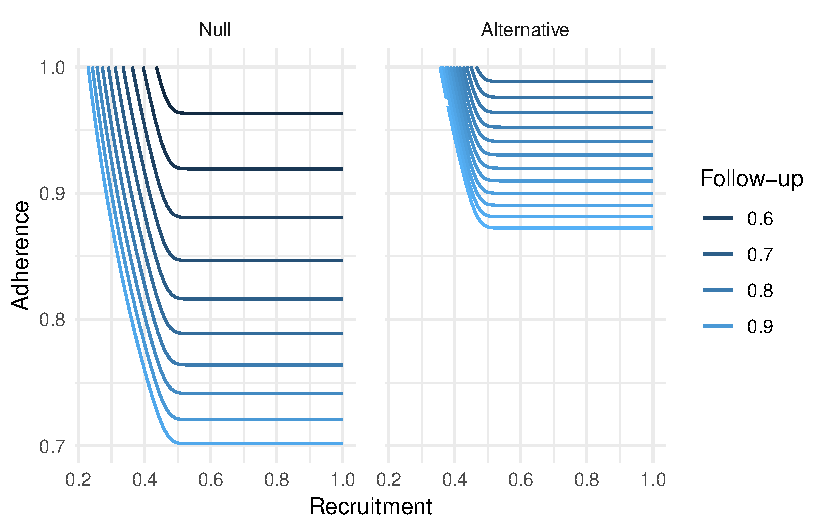
\includegraphics[scale=0.8]{./Figures/hyps.pdf}
\caption{Values of recruitment, follow-up and adherence parameters for leading to a definitive trial power of $p_0 = 0.6$ (i.e. the boundary of the null hypothesis, left panel), or $p_1 = 0.8$ (i.e. the boundary of the alternative hypothesis, right panel).}
\label{fig:hyps}
\end{figure}

Given the hypotheses and assuming follow-up and adherence outcomes are independent, we solved the optimisation problem described in Section \ref{sec:ocs} to obtain operating characteristic curves for pilot sample sizes of $n_p = 30, 50, 100$ per arm. As shown in Figure \ref{fig:ex_ocs}, operating characteristics with the original sample size of $n_p = 30$ are in the region of nominal values typically seen in phase II drug trials. For example, a power of $1-\beta \approx 0.83$ is possible with a type I error rate of $\alpha \approx 0.1$. As would be expected, error rates can be significantly reduced by increasing the pilot sample size. For example, setting $n_p = 50$ can increase power to around 0.95 whilst maintaining type I error at $\alpha \approx 0.1$.

\begin{figure}
\centering
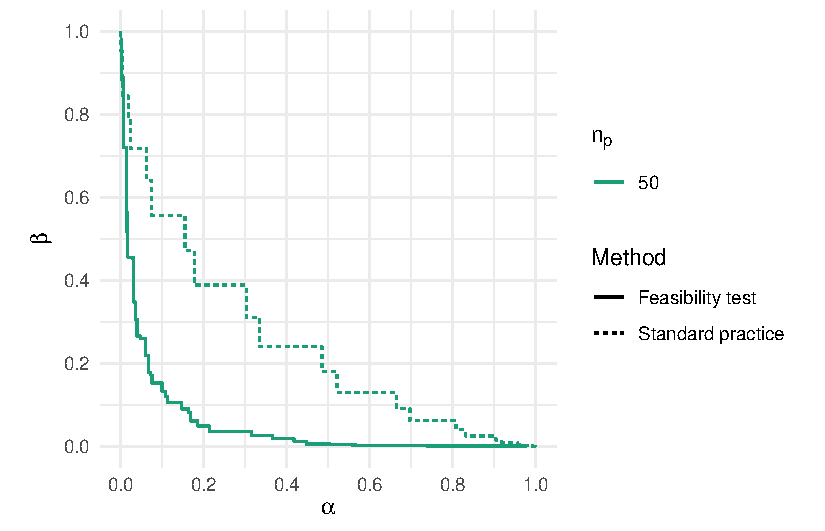
\includegraphics[scale=0.8]{./Figures/ex_ocs.pdf}
\caption{Type I ($\alpha$) and type II ($\beta$) error rates obtained for a range of critical values $c$ and pilot sample sizes $n_p$ when using the proposed method (solid lines). Error rates available when using conventional progression criteria and for a pilot sample size of $n_p = 50$ are shown for comparison (dashed line).}
\label{fig:ex_ocs}
\end{figure}

% Comparison
To provide a comparison with the proposed method, we also calculate the error rates available using the standard approach to setting progression criteria. That is, we considered decision rules based on three critical values $c_f, c_a$ and $c_r$, where we proceed to the definitive trial only when $\hat{\phi}_f > c_f$, $\hat{\phi}_a > c_a$ and $\hat{\phi}_r > c_r$. Continuing to assume independence between the parameter estimates, the probability of this event is then
\begin{align*}
Pr[\text{go} ~ | ~ \phi] &= Pr[\hat{\phi}_r > c_r ~ | ~ \phi] \times Pr[ \hat{\phi}_f > c_f ~ | ~ \phi] \times Pr[ \hat{\phi}_a > c_a ~ | ~ \phi] \\
&= F_{r_-}( 2n_p/c_r - 2n_p ~ | ~ \phi) \times [1-F_f(2n_p c_f ~ | ~ \phi)] \times [1-F_a(n_p c_a ~ | ~ \phi)],
\end{align*}
Where $F_{r_-}(.), F_f(.)$ and $F_a(.)$ are the cumulative distribution functions for the random variables $R_-, F$ and $A$ in the pilot, respectively. We calculated the error rates available for a pilot sample size of $n_p = 50$ by extending the optimisation problem described in Section \ref{sec:ocs} to search over the space of the three critical values  $c_f, c_a$ and $c_r$. Formally, we solved

\begin{alignat*}{1}
\max ~ & \left(h(n_p, c, \phi_0) , ~ 1 - h(n_p, c, \phi_1) \right) \\
\text{subject to} ~ & (c_r, a_a, c_f) \in [0,1]^3, \\
& \phi_0 \in \Phi_0, \\
& \phi_1 \in \Phi_1. 
\end{alignat*}

Figure \ref{fig:ex_ocs} shows that, regardless of the PC thresholds used, the procedure is very inefficient in comparison to the proposed test. For example, recall that the proposed test can give a power of around 0.95 for a type I error rate of around 0.1. Using the standard approach and maintaining the same type I error rate, power is reduced to around 0.35.

An alternative view which may be helpful when designing the pilot trial is to examine the probability of proceeding to the definitive trial as a function of $p_0$, the power used to define the null hypothesis. If $p_1$ is kept fixed at, say, $p_1 = 0.8$, we can identify the critical value which will give a certain desired type II error rate in the pilot. This is illustrated in Figure \ref{fig:eval2}, which shows how the type I error rate of the pilot increases as $p_0$ increases for $n_p = 30, 50, 100$, keeping the type II error rate fixed all the while at 0.1. This view shows that, for example, while a large pilot sample of $n_p = 100$ will ensure we will never proceed to a definitive trial with a true power of $p_0 = 0.6$ is 0, it will also mean that when $p_0 = 0.75$ there will be no more that a 0.5 chance of proceeding. This might be considered rather low, when we have defined the alternative hypothesis using $p_1 = 0.8$. In comparison, the associated values when $n_p = 50$ are around 0.08 and 0.75.

\begin{figure}
\centering
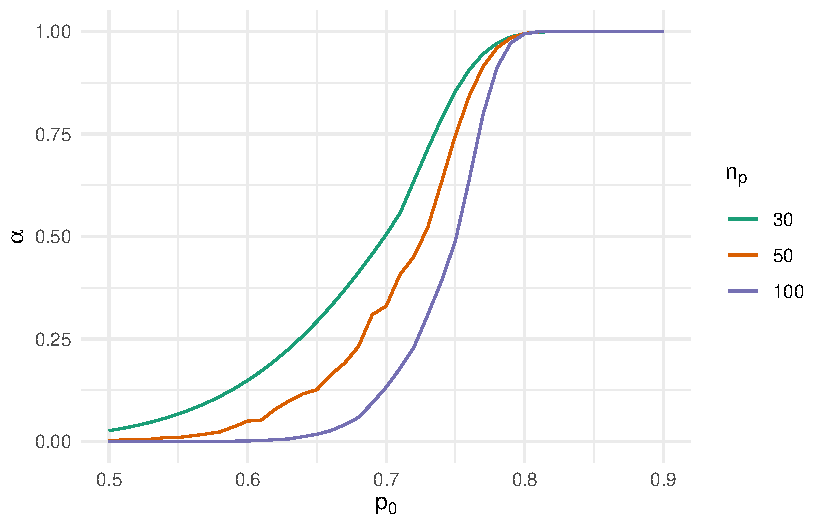
\includegraphics[scale=0.8]{./Figures/eval2.pdf}
\caption{Type I error rates for pilot trials of different sample sizes $n_p$, as a function of the null hypothesis parameter $p_0$ and keeping type II error maintained at 0.1.}
\label{fig:eval2}
\end{figure}

\section{Evaluation}\label{sec:eval}

%Note that n_e, n_t, mu and sd only come into things when defining the hypotheses. looking at x(phi), we have a term mu*E[n]/sd (if we take the first term in the denominator to dominate the second). if phi_r is large enough, E[n] = n_t and n_e disappears. Empirically, we find that error rates are maximised when phi_r is large enough. So the problem only changes with the factor n_t*mu/sd, i.e. we only need to change one of the variables while keeping the other two fixed, as we do in the evaluation.

To understand the properties of the proposed method more generally, we calculated the error rates available under 9 scenarios with different target sample size ($n_t = 235, 258, 282$) and powers defining the null hypothesis ($p_0 = 0.6, 0.65, 0.7$). Throughout, the power defining the alternative hypothesis was kept at $p_1 = 0.8$, and the effect size at $\mu = 0.3$, the standard deviation at $\sigma = 1$ and the number of eligible participants at $n_e = 500$. The target sample sizes were determined by first calculating the number needed to give the definitive trial a power of 90\% under perfect follow-up and adherence, and then inflating this by 10 and 20\% to allow for some anticipated imperfection in these parameters. For each scenario we calculated the operating characteristics of a pilot with sample size $n_p = 30, 50, 100$.

%Operating characteristics are not affected by the value of $n_e$ (why? explain), so this was kept constant at 500. They are affected by the standardised effect size to be detected, $\mu/\sigma$, and the target sample size $n_t$, but only through their the power obtained by that sample size for that effect. So, we keep the standardised effect size constant at 0.3, and vary $n_t$. These numbers are obtained by first calculating the sample size required to give 90\% power in the ideal scenario of complete adherence and follow-up, and then inflating to allow for some discrepancies. We inflate by 0, 10 and 20\%. 
 
%results
The resulting error rates are illustrated in Figure \ref{fig:eval}. We see that inflating the target sample size leads to a small increase in error rates. For example, for $n_p = 30$, $n_t = 234$ and $p_0 = 0.7$ (top right panel), the pilot can have error rates of $\alpha = 0.094$ and $\beta = 0.557$. Increasing the target sample size to $n_t = 281$ gives an increased type II error rate of $\beta = 0.682$ whilst approximately maintaining type I error, with $\alpha = 0.097$. This general behaviour can be explained by noting that more recruited participants will mean we can tolerate worse follow-up and/or adherence whilst maintaining power, so the hypotheses will expand , and in general we can expect error rates to increase as the size of the hypotheses they are defined over increase. Error rates are more sensitive to the power used to define the null hypothesis. For example, with $n_p = 30$ and $p_0 = 0.7$ one can obtain error rates of $\alpha = 0.094$ and $\beta = 0.557$. If we reduce $p_0$ to 0.6, increasing the distance between the hypotheses, one can reduce type II error to $\beta = 0.14$ in exchange for a negligible increase in type I error to $\alpha = 0.099$. The proposed method substantially outperforms the conventional approach in all scenarios, with the latter in some cases proving to be less effective than tossing a (possibly biased) coin as a means of making a stop/go decision (when $p_0 = 0.7$, right column). The stepped nature of the operating characteristic curves, which becomes more pronounced as the pilot sample size decreases, results from the binary nature of the three endpoints under consideration.

\begin{figure}
\centering
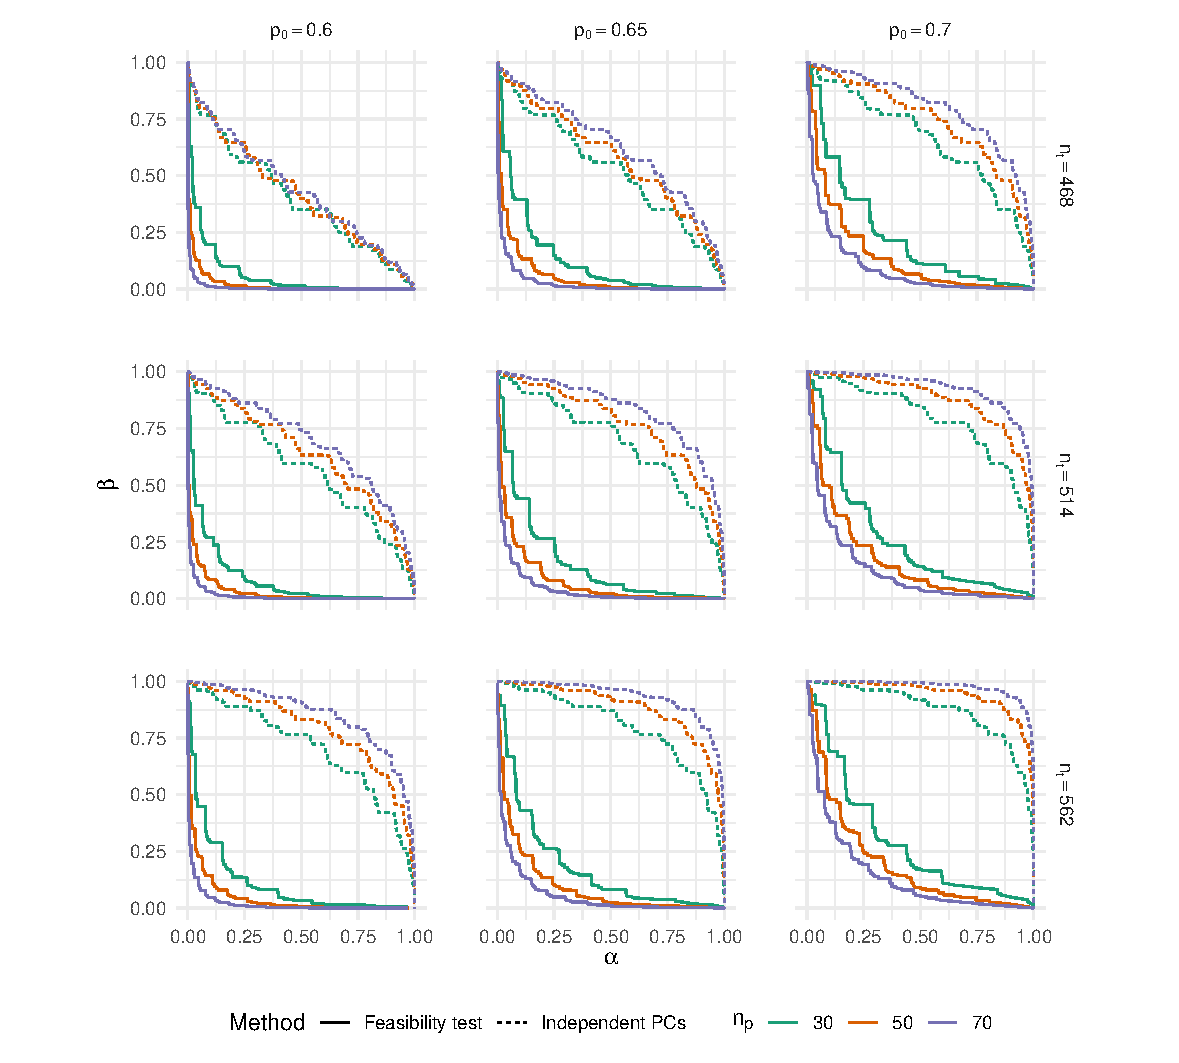
\includegraphics[scale=0.8, trim={1.5cm 0 0 0},clip]{./Figures/eval.pdf}
\caption{Type I ($\alpha$) and type II ($\beta$) error rates obtained for a range of critical values $c$ and pilot sample sizes $n_p$ when using the proposed method (solid lines) and the conventional approach (dashed line). The power used to define the null hypothesis increases from left to right, $p_0 = 0.6, 0,65, 0.7$, while the target sample size of the definitive trial is increased from top to bottom, $n_t = 235, 258, 282$.}
\label{fig:eval}
\end{figure}

\section{Extension - unknown variance}\label{sec:extension}

Thus far we have considered how recruitment, follow-up and adherence rates all affect the power of the definitive trial, and have shown how these can be assessed in the pilot trial as part of a hypothesis test. Another parameter which affects the power of the definitive trial is the standard deviation of the outcome measure: recall from Section \ref{sec:power} that the conditional power is 
\begin{equation*}
g(\phi, \sigma) = \Phi \left( x(\phi, \sigma) - z_{1-\alpha} \right),
\end{equation*}
where 
$$
x(\phi, \sigma) =  \frac{ \phi_a\mu \sqrt{\phi_f E[R]} } {\sqrt{2\sigma^2 + \mu^2 \phi_a(1-\phi_a)}}.
$$
An estimate of the standard deviation obtained in the pilot, $\hat{\sigma}$, can therefore be included in the pilot statistic $s(\hat{\phi}, \hat{\sigma}) = x(\hat{\phi}, \hat{\sigma})$ to allow for high variability in the outcome measure, which may lead to a trial with infeasibly low power, to be identified in the pilot.

For notational simplicity and ease of computation we will focus on the case where follow-up and adherence are independent, but the method will extend naturally to the more general case. The power of the pilot trial is now approximately 
\begin{align*}
h(n_p, c, \phi, \sigma) &= \sum_{n_{af}} \left( \sum_{r^- = 0}^{r^-_{max}} 
\left[ \int_0^y p_{\sigma^2}(x(\phi) | r^-, n_{af}, \phi) \right] p_{r^-}(r^- | n_{af}, \phi) \right)     
p_{af}(n_{af} |\phi).
\end{align*}
The integral is the c.d.f. of the sample variance's sampling distribution, which is
$$
\hat{\sigma}^2 \sim \frac{\sigma^2 \chi^2_{2n_p\hat{\phi}_f - 1}}{2n_p\hat{\phi}_f - 1}.
$$
The upper limit is
$$
y = \frac{\hat{\phi}_f \hat{\phi}_a^2 \mu^2 \hat{E[N]} - \mu^2 \hat{\phi}_a (1-\hat{\phi}_a) c}{2c^2}.
$$

Empirically, we find that both type I and II error rates increase as the standard deviation decreases. To avoid the trivial situation where error rates tend to 1 as $\sigma$ tends to zero, we include a lower limit on $\sigma_*$ in the definitions of the hypotheses $\Phi_0$ and $\Phi_1$, giving
\begin{align*}
\Phi_0 &= \{\phi \in \Phi, \sigma > \sigma_*  ~ | ~ g(\phi, \sigma) <= p_0 \}; \\
\Phi_1 &= \{\phi \in \Phi, \sigma > \sigma_* ~ | ~ g(\phi, \sigma) >= p_1 \}.
\end{align*}

To illustrate the effect of allowing for uncertainty in $\sigma$, we calculated the error rates available when $n_p = 30, n_t = 235, p_0 = 0.6$ and $p_1 = 0.8$, and the lower limit was taken to be $\sigma_* = 0.8$. We can then compare these error rates with those previously obtained when it was assumed that $\sigma = 1$. Figure \ref{fig:unknown_var} illustrates the impact of relaxing the assumption. For example, recall that when $\sigma$ was assumed known, a pilot trial type I error rate of around 0.1 allowed a type II error rate of around 0.14. Maintaining the same type I error but now estimating $\sigma$ in the pilot increases type II error to 0.51. The detriment stems from two issues. Firstly, by using the pilot estimate in the test statistic $s(\hat{\phi}, \hat{\sigma})$ its sampling variability is increases. Secondly, by allowing for the lower limit of $\sigma_* = 0.8$ we accommodate lower values of the rates $\phi_r, \phi_a$ and $\phi_f$ in our hypotheses in much the same way as in Section \ref{sec:eval} when we increased $n_t$, with the same effect of enlarging the hypotheses and thus allowing more extreme error rates to be located.

\begin{figure}
\centering
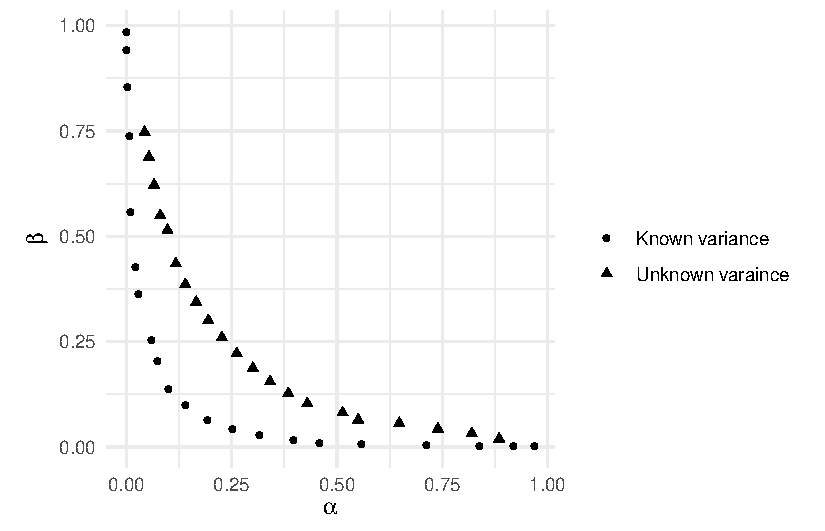
\includegraphics[scale=0.8]{./Figures/unknown_var.pdf}
\caption{Type I ($\alpha$) and type II ($\beta$) error rates obtained for a range of critical values $c$ and pilot sample size $n_p = 30$ when the standard deviation of the primary outcome is either assumed known or estimated in the pilot trial.}
\label{fig:unknown_var}
\end{figure}

\section{Discussion}

We have proposed a statistical test which simultaneously assesses recruitment, follow-up and adherences rates in order to anticipate and mitigate related problems which would render the planned definitive trial infeasible. We have shown that, without increasing the sample size of the pilot trial beyond typical values, the test can lead to good operating characteristics in terms of type I and II errors. Moreover, we have shown these to be a substantial improvement on those resulting from applying the conventional approach to setting progression criteria in pilot trials. We have shown how the test can be extended to include the common pilot objective of estimating an unknown standard deviation nuisance parameter, and found that for this to be incorporated the sample size of the pilot trial may have to be increased.

\subsection{Relation to existing literature}

In a sense, the suggestion of testing hypotheses in pilots goes against the current guidance warning that tests are likely to be severely underpowered. However, it should be emphasised that the standard practice of pre-specifying several progression criteria and proceeding to the definitive trial only if the corresponding pilot estimates exceed their thresholds is equivalent to a intersection hypothesis test of multiple endpoints. Yet, without any appropriate hypotheses defined, we cannot determine the error rates of such an intersection test. Moreover, we have shown that in some cases it would be impossible to obtain reasonable error rates, regardless of the threshold values used in the PCs. We may have anticipated this, given that intersection tests suffer from the so-called `reverse multiplicity' problem which tends to lead to low power. Thus, even if the proposed method is not deemed to be appropriate for a specific pilot trial, we have demonstrated that a formal statistical analysis of any proposed PCs should be carried out before they are decided upon.

One benefit of the proposed method is that it provides a rationale for the choice of sample size. This is an area in need of methodological attention. Almost all methods for pilot trials only consider the problem of obtaining a sufficiently precise estimate of the SD, and there is no reason to think this will be sufficient for other quantitative pilot objectives. The methods available are often reduced down to simple rules-of-thumb, in some cases incorrectly (i.e. miss-attribution of Browne). The popularity of these one-size-fits-all approaches is perhaps reflective of the difficulty researchers face when trying to do anything more principled. Although the sample size of pilots is often justified by reporting the anticipated precision in the estimates of feasibility parameters (e.g. the widths of confidence intervals), there is no clear guidance on how precise they should be, or how to weigh precision against the cost of sampling.

\subsection{`Amber' decisions}

Our method leads to a binary stop/go decision. Increasingly, progression criteria in pilot trials are incorporating three outcomes, adding an additional intermediate `amber' decision between the `red' stop and `green' go \cite{Avery2017}. The intention is that if the pilot estimate is neither clearly good nor bad, but somewhere between, then it may be possible to make some modifications to the intervention or the trial protocol which would ensure the definitive trial will be feasible. If the effect of these modifications were known in advance (for example, the effect on recruitment of opening another centre), this process could potentially be modelled at the pilot design stage and its effect on pilot operating characteristics captured. We might expect this to be infeasible in general, though, as the nature and magnitude of modiifications will not in general be known until after the pilot has been completed. An example referred to in \cite{Avery2017} is of a trial manager being absent on sick leave for much of the pilot. Once this has been identified we might reasonably expect a large improvement in the recruitment rate in the definitive trial if measures to ensure cover of trial managers are put in place; but it would have been impossible to know, prior to the pilot, that such an effect was going to be available. This is important under the hypothesis testing paradigm we have used in this paper, where all decision rules must be pre-specified and should be adhered to.

In practice, the pilot trial could be designed using our method and assuming no modifications will be possible, and, in the event that we wish to make modifications, another pilot could be done to assess the effect of these. This would appear to be in line with the MRC framework for complex intervention development and evaluation \cite{Craig2008}, although we are not ware of any examples where two or more pilots have been done in preparation for a definitive trial. Alternatively, if the modifications are made and we proceed directly to the definitive trial, we should be clear that the error rates associated with the pilot trial as designed will no longer apply. Even in the idealised scenario of knowing exactly what the effect of the modification will be, due to the binary nature of the endpoints being assessed in the pilot, error rates will not remain constant if hypotheses and critical values are shifted by the same amount. For example, consider a very simple example where we test one binary endpoint with parameter $\rho$ and our original null and alternative hypotheses are $\rho_0 = 0.7, \rho_1 = 0.8$ with a decision rule of proceeding if and only if $\hat{\rho} > 0.75$. If we become aware that we can modify the intervention and increase the parameter value by 0.2, we may want to shift the hypotheses to $\rho_0 = 0.5, \rho_1 = 0.6$ and decision rule to $\hat{\rho} > 0.75$. However, for a sample size of 60 being used to estimate $\rho$, this transformation will increase the type I error from 0.20 to 0.22 and type II error from 0.17 to 0.21. In the more realistic case where the modification effect is estimated with some error as opposed to known exactly, the error rates will deviate from the original numbers even more. A Bayesian approach may be the solution to these issues, since there is no requirement to observe pre-specified decision rules, and instead any beliefs about modification effects can be incorporated into the parameter distributions which can in turn be used to inform decision making. Finally, we note that although some methods proposed in the phase II drug trial setting have allowed for three outcomes \cite{Sargent2001, Hong2007}, they are designed to allow for other non-primary endpoints to influence the stop/go decision, not to allow for any modifications.

\subsection{Fixing the definitive trial design}

We have assumed throughout that the definitive trial sample size is fixed and will not be changed after the pilot trial, which may be considered restrictive in practice. For example, consider a scenario where the alternative hypothesis was defined as those parameters which would give a power of at least $p_1 = 0.8$ given the intended sample size of $n = 234$. The pilot test only just exceeds the critical value, thus suggesting a `go' decision, but the pilot estimates predict that the power of the main trial will be 0.7 if $n = 234$. Using the pilot estimates, we calculate that the definitive trial sample size should be increased to $n = 298$ to obtain a power of 0.8. Such actions are permissible when using the proposed test, providing the interpretation of the hypotheses and error rates are clarified. 

Figure \ref{fig:adjust_n} illustrates the preceding example, showing the power curves associated with the null and alternative hypotheses together with that associated with the critical value. Note that the maximum inflation to the sample size we would ever consider is to $n=298$, since any pilot estimates which lie below the critical value curve (and would thus require $n > 234$ for 0.8 power) would be rejected by the test. We can therefore consider the result of the procedure to be a sample size $n \in [234, 298]$ as shown in Figure \ref{fig:adjust_n}. We can now think about null and alternative hypotheses as the segments of the illustrated power curves in this range. That is, we consider a definitive trial with $n = 298$ and power $\approx 0.70$ to be in the null hypothesis, such that if it were to be realised we would consider it a type I error. Similarly, not proceeding to a definitive trial with $n=298$ and power $\approx 0.89$ would be considered a type II error. Given the approximately linear nature of the power curves we could interpret the approximate slope as a linear trade-off between sample size and power, in the sense that the benefit of an increase in power of around 0.1 is cancelled out by an increase in the sample size of 64.

\begin{figure}
\centering
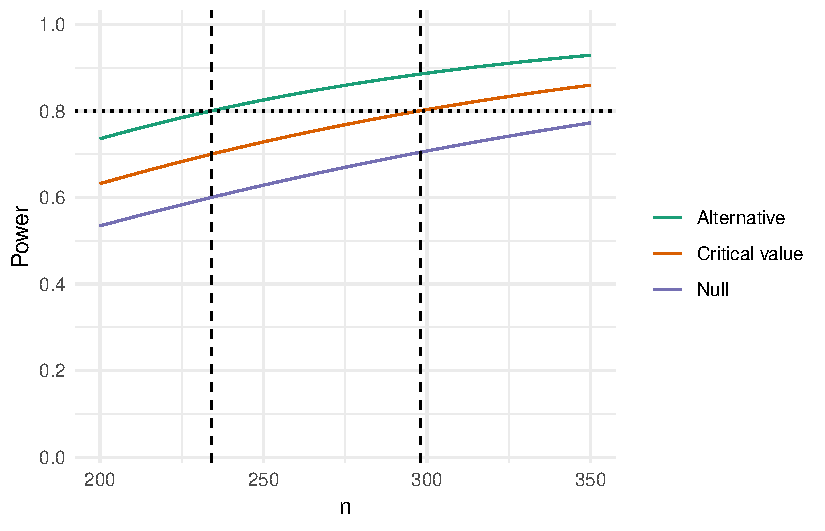
\includegraphics[scale=0.8]{./Figures/adjust_n.pdf}
\caption{Adjusting n.}
\label{fig:adjust_n}
\end{figure}

\subsection{Extending to other types of trial designs}

We have focussed on a specific problem where the definitive trial will have a randomised two-arm design and has a single, normally distributed primary outcome measure. Our method could be applied directly to any variant of this problem. For example, a binary endpoint can be incorporated using a normal approximation if the definitive trial sample size is sufficiently large; or a cluster randomised trial could be addressed if the endpoints are all measured at the cluster level. To extend the method to other problems, we would require an expression for the power of the definitive trial (as a function of parameters $\phi$), a statistic to use in the pilot trial, and an expression for the power of the pilot trial using that statistic. When analytic forms of the power functions cannot be found, they can be approximated using simulation \cite{Landau2013} and, in principle, the optimisation problem \ref{eqn:MO_opt} could be solved as before. In practice, evaluating the two objectives and two constraints of \ref{eqn:MO_opt} using simulation would be computationally demanding and infeasible using the same NSGA-II algorithm. Future work could explore how efficient global optimisation algorithms \cite{Jones2001} could be used to solve these problems in a timely manner 

\subsection{Assessing potential efficacy}

In addition to the recruitment, follow-up and adherence rates and the standard deviation we have considered in this paper, another parameter which would be of interest when deciding to run a definitive trial is the treatment effect $\mu$. We could consider incorporating $mu$ into our method, including it in our hypotheses definitions and its estimate into the pilot test statistic, but there are at least two methodological challenges in doing so. Firstly, as we increase the effect $\mu$ when defining our hypotheses, we will accommodate worse values of the remaining parameters whilst maintaining power. To avoid trivial cases where, for example, a follow-up rate of $\phi_f$ is considered acceptable because the treatment effect is so large, a upper limit on $\mu$ would have to be specified when defining the hypotheses. Because error rates are likely to be maximised at this extreme value, operating characteristics will likely be highly sensitive to the choice of the limit.

A second issue is that, unlike parameters like follow-up rate, the treatment effect is not of interest only in as much as it effects the power of the definitive trial. For example, two points in the parameter space could lead to the same power, but one may be considered in the null and the other in the alternative because the treatment effect in the latter is so much greater. With several attributes of interest (in this case, power and treatment effect), one potentially useful avenue for future research is the use of Bayesian statistical decision theory. In addition to allowing a utility function which would allow the preferences and trade-offs between multiple attributes to be fully articulated, working in a Bayesian framework would also allow us to focus attention on plausible regions of the parameter space as opposed to extreme points, thus helping to address the first issue.

\subsection{Other}

A criticism of the proposed method is the simplicity of the decision rule it suggests. Particularly in the case of pilot trials of complex interventions, we would expect the decision of if and how the definitive trial should be conducted to be informed by many factors beyond the pilot estimates of a handful of parameters, not least qualitative outcomes. However, we believe the method will still provide a useful guide to decision making, and allows for the choice of pilot sample size to be considered more fully. This view is supported by the continued prevalence of N-P hypothesis testing for the design and analysis of all types of clinical trials, where the final decision is rarely made by following the result of the test.

The proposed method could benefit from further methodological research. The proposed statistic is not guaranteed to be optimal in any sense (e.g. uniformly most powerful), and so further research could consider alternatives and their properties. In the case of unknown variance, we found empirically that error rates are maximised when the true standard deviation was equal to the lower bound. If this were found to hold in general, the optimisation problem of maximising error rates would be simplified and thus solvable in a shorter time.

\ack
Acknowledgements.

%\bibliographystyle{unsrt}
\bibliography{U:/Literature/Databases/DTWrefs}

\appendix
%\section*{Derivations}

We derive the variances of the group means in the definitive trial as given in equation \ref{eqn:vars}. By the law of total variance,
\begin{equation}\label{eqn:int_group_mean}
Var(\bar{Y}_1) = E[Var(\bar{Y}_1 | F_1, A)] + 
E[Var(E[\bar{Y}_1 | F_1, A] | F_1)] + 
Var(E[\bar{Y}_1 | F_1]).
\end{equation}
Taking each of these terms in turn:
$$
E[Var(\bar{Y}_1 | F, A)] = E \left[ \frac{\sigma^2}{F_1} \right] = \frac{\sigma^2}{\phi_f E[R]},
$$
where $E[R]$ is the expected number of participants recruited in the intervention arm. Recall that we denote the number of eligible participants who consent by $C$. Then,
$$
E[R] = E[R ~|~ C < n_t] Pr(C < n_t) + E[R ~|~ C \geq n_t] Pr(C \geq n_t).
$$
Note that $C$ follows a binomial distribution with size $n_e$ and probability $\phi_r$. Clearly, $E[R ~|~ C \geq n_t] = n_t$. We also have
$$
E[R ~|~ C < n_t] = \frac{\sum_{k=0}^{n_t-1} k{n_e \choose k} \phi_r^k (1-\phi_r)^{n_e - k} } {Pr(C < n_t)},
$$
and so 
$$
E[R] = \sum_{k=0}^{n_t-1} k{n_e \choose k} \phi_r^k (1-\phi_r)^{n_e - k} + n_t Pr(C \geq n_t).
$$

Returning to equation \ref{eqn:int_group_mean}, the second term is 
\begin{align*}
E \left[ Var(E[\bar{Y}_1 | F_1, A] ~|~ F_1) \right] &= E \left[ Var \left(\frac{A\mu}{F_1} ~|~ F_1 \right) \right] \\
&= E \left[\frac{\mu^2}{F_1^2} Var(A ~|~ F_1) \right] \\
&= E \left[ \frac{\mu^2}{F_1^2} F_1 \phi_a (1-\phi_a) \right] \\
&= \frac{\mu^2}{\phi_f E[R]} \phi_a (1-\phi_a).
\end{align*}
Finally,
\begin{align*}
Var(E[\bar{Y}_1 | F_1]) &= Var \left( E \left[ A ~|~ F_1 \right] \frac{\mu}{F_1} \right) \\
&= Var \left( F_1 \phi_a \frac{\mu}{F_1} \right) \\
&= 0.
\end{align*}
This then gives
$$
Var(\bar{Y}_1) = \frac{\sigma^2}{\phi_f E[R]} + \frac{\mu^2}{\phi_f E[R]} \phi_a (1-\phi_a).
$$

For the control group the sample mean will be $\bar{Y}_0 = \frac{1}{F_0}\sum_{i=1}^{F_0} e_i$. Its expectation is 0, and its variance is
\begin{align*}
Var(\bar{Y}_0) &= E[Var(\bar{Y}_0 | F_0)] + Var(E[\bar{Y}_0 | F_0]) \\
&= E \left[ \frac{\sigma^2}{F_0} \right] + 0\\
&= \frac{\sigma^2}{\phi_f E[R]}.
\end{align*}


\end{document}
